\documentclass[otchet]{SCWorks}
% Тип обучения (одно из значений):
%    bachelor   - бакалавриат (по умолчанию)
%    spec       - специальность
%    master     - магистратура
% Форма обучения (одно из значений):
%    och        - очное (по умолчанию)
%    zaoch      - заочное
% Тип работы (одно из значений):
%    coursework - курсовая работа (по умолчанию)
%    referat    - реферат
%  * otchet     - универсальный отчет
%  * nirjournal - журнал НИР
%  * digital    - итоговая работа для цифровой кафедры
%    diploma    - дипломная работа
%    pract      - отчет о научно-исследовательской работе
%    autoref    - автореферат выпускной работы
%    assignment - задание на выпускную квалификационную работу
%    review     - отзыв руководителя
%    critique   - рецензия на выпускную работу

% * Добавлены вручную. За вопросами к @mchernigin
\usepackage{preamble}
\floatplacement{figure}{H}
%\setkeys{Gin}{width=1.0\textwidth}
\setminted{breaklines=true, breakanywhere=true}

\begin{document}

% Кафедра (в родительном падеже)
\chair{математической кибернетики и компьютерных наук}

% Тема работы
\title{Создание представлений в базе данных и работа с ними}

% Курс
\course{3}

% Группа
\group{351}

% Факультет (в родительном падеже) (по умолчанию "факультета КНиИТ")
\department{факультета компьютерных наук и информационных технологий}

% Специальность/направление код - наименование
% \napravlenie{02.03.02 "--- Фундаментальная информатика и информационные технологии}
% \napravlenie{02.03.01 "--- Математическое обеспечение и администрирование информационных систем}
% \napravlenie{09.03.01 "--- Информатика и вычислительная техника}
\napravlenie{09.03.04 "--- Программная инженерия}
% \napravlenie{10.05.01 "--- Компьютерная безопасность}

% Для студентки. Для работы студента следующая команда не нужна.
\studenttitle{студентки}

% Фамилия, имя, отчество в родительном падеже
\author{Потапкиной Маргариты Андреевны}

% Заведующий кафедрой 
\chtitle{доцент, к.\,ф.-м.\,н.}
\chname{С.\,В.\,Миронов}

% Руководитель ДПП ПП для цифровой кафедры (перекрывает заведующего кафедры)
% \chpretitle{
%     заведующий кафедрой математических основ информатики и олимпиадного\\
%     программирования на базе МАОУ <<Ф"=Т лицей №1>>
% }
% \chtitle{г. Саратов, к.\,ф.-м.\,н., доцент}
% \chname{Кондратова\, Ю.\,Н.}

% Научный руководитель (для реферата преподаватель проверяющий работу)
\satitle{доцент, к.\,ф.-м.\,н.}
\saname{И.\,А.\,Батраева}

% Руководитель практики от организации (руководитель для цифровой кафедры)
\patitle{доцент, к.\,ф.-м.\,н.}
\paname{И.\,А.\,Батраева}

% Руководитель НИР
\nirtitle{доцент, к.\,п.\,н.} % степень, звание
\nirname{И.\,А.\,Батраева}

% Семестр (только для практики, для остальных типов работ не используется)
\term{5}

% Наименование практики (только для практики, для остальных типов работ не
% используется)
\practtype{учебная}

% Продолжительность практики (количество недель) (только для практики, для
% остальных типов работ не используется)
\duration{2}

% Даты начала и окончания практики (только для практики, для остальных типов
% работ не используется)
\practStart{01.07.2024}
\practFinish{13.01.2024}

% Год выполнения отчета
\date{2026}

\maketitle

% Включение нумерации рисунков, формул и таблиц по разделам (по умолчанию -
% нумерация сквозная) (допускается оба вида нумерации)
\secNumbering

\tableofcontents

% Раздел "Обозначения и сокращения". Может отсутствовать в работе
% \abbreviations
% \begin{description}
%     \item ... "--- ...
%     \item ... "--- ...
% \end{description}

% Раздел "Определения". Может отсутствовать в работе
% \definitions

% Раздел "Определения, обозначения и сокращения". Может отсутствовать в работе.
% Если присутствует, то заменяет собой разделы "Обозначения и сокращения" и
% "Определения"
% \defabbr

\intro
В ходе выполнения работы были изучены различные виды представлений в базе данных. Были созданы несколько обычных представлений; обновляемые представления с конструкцией WITH CHECK OPTION, в частности обновляемые представления, основанные на других представлениях с использованием LOCAL и CASCADED CHECK OPTION; материализованное представление и индекс для него с целью сравнения производительности.

\section{Обычные представления}

Задание было выполнено по следующему плану:

\begin{enumerate}
\item Создать представление.
\item Написать запрос SELECT для проверки того, что представление возвращает только требуемые данные.
\item Получить код созданного представления.
\end{enumerate}

\subsection{Представление для преподавателей (view\_teachers)}

\begin{enumerate}
\item Код представления:
\begin{minted}{sql}
CREATE OR REPLACE VIEW view_teachers AS
SELECT
  teachers.surname AS teacher_surname,
  teachers.name AS teacher_name,
  teachers.patronymic AS teacher_patronymic,
  departments.name AS department_name
FROM teachers
RIGHT JOIN departments
ON teachers.id = departments.head_teacher_id;
\end{minted}

\item Запрос к представлению и его результат:
\begin{minted}{sql}
SELECT * FROM view_teachers LIMIT 10;
\end{minted}

\begin{figure}
\centering
    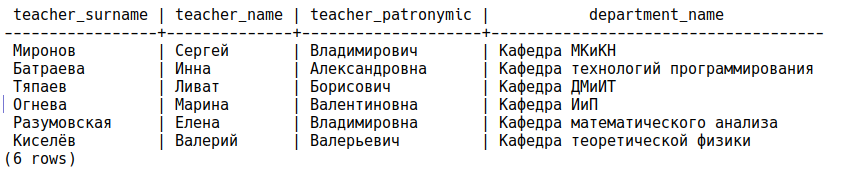
\includegraphics[scale=0.8]{q1p1.png}
\end{figure}

\item Получение кода представления:
\begin{minted}{sql}
SELECT pg_get_viewdef('view_teachers', true);
\end{minted}

\begin{figure}
\centering
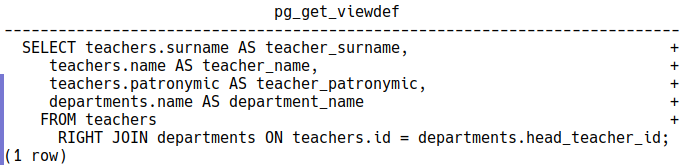
\includegraphics{q1p2.png}
\end{figure}
\end{enumerate}

\subsection{Представление для оценок (view\_marks)}

\begin{enumerate}
\item Код представления:
\begin{minted}{sql}
CREATE OR REPLACE VIEW view_marks AS
SELECT
  students.name AS student_name,
  students.surname AS student_surname,
  grades.points,
  COALESCE (grades.mark::VARCHAR, 'зачёт') AS mark,
  subjects.name AS subject_name
FROM grades
INNER JOIN students ON grades.student_id = students.id
INNER JOIN study_plan_subject ON grades.study_plan_subject_id = study_plan_subject.id
INNER JOIN subjects ON study_plan_subject.subject_id = subjects.id
WHERE students.is_expelled = FALSE;
\end{minted}

\item Запрос к представлению и его результат:
\begin{minted}{sql}
SELECT * FROM view_marks LIMIT 20;
\end{minted}

\begin{figure}
\centering
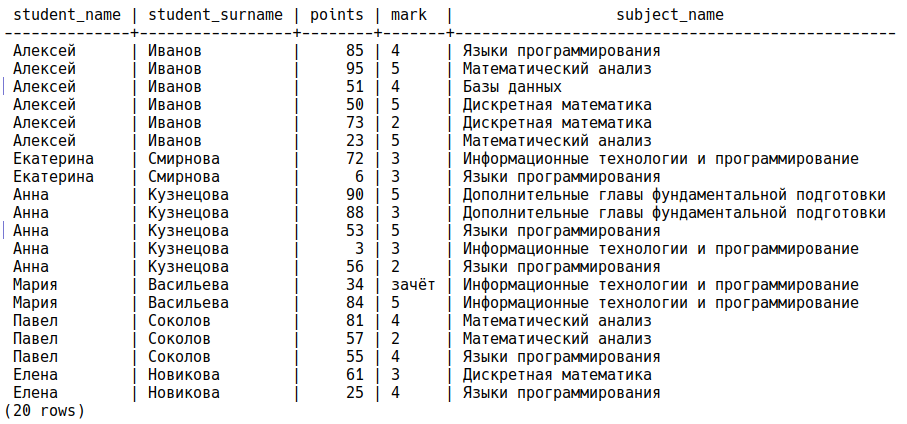
\includegraphics[scale=0.8]{q2p1.png}
\end{figure}

\item Получение кода представления:
\begin{minted}{sql}
SELECT pg_get_viewdef('view_marks', true);
\end{minted}

\begin{figure}
\centering
    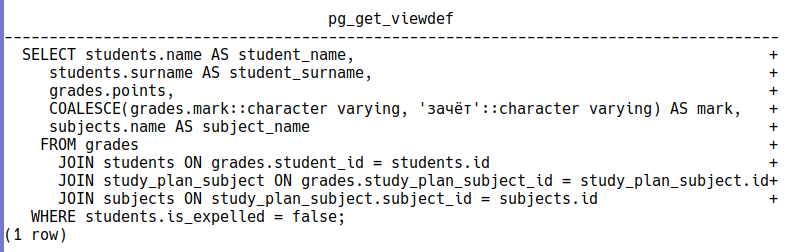
\includegraphics[scale=0.8]{q2p2.png}
\end{figure}
\end{enumerate}

\subsection{Представление для структуры университетов (view\_structure)}

\begin{enumerate}
\item Код представления:
\begin{minted}{sql}
CREATE OR REPLACE VIEW view_structure AS
SELECT
  REPLACE (departments.name, 'Кафедра', 'Подразделение') AS department_name,
  faculties.name AS faculty_name,
  universities.name AS university_name
FROM departments
INNER JOIN faculties ON faculties.id = departments.faculty_id
INNER JOIN universities ON universities.id = faculties.university_id;
\end{minted}

\item Запрос к представлению и его результат:
\begin{minted}{sql}
SELECT * FROM view_structure LIMIT 10;
\end{minted}

\begin{figure}
\centering
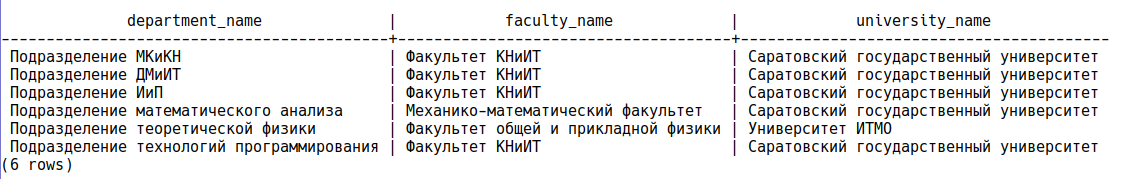
\includegraphics[scale=0.6]{q3p1.png}
\end{figure}

\item Получение кода представления:
\begin{minted}{sql}
SELECT pg_get_viewdef('view_structure', true);
\end{minted}

\begin{figure}
\centering
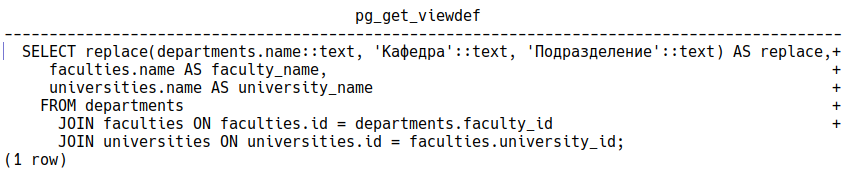
\includegraphics[scale=0.7]{q3p2.png}
\end{figure}
\end{enumerate}

\section{Обновляемые представления}
Обновляемое представление позволяет изменять данные в зависимых таблицах. Обновление или вставка данных с помощью представления, в котором задана конструкция WITH CHECK OPTION, осуществляется, только если строка, полученная в результате применения этой операции обновления или вставки, соответствует критериям, допускающим ее включение в это представление. 

\subsection{Обычное обновляемое представление}
\begin{enumerate}
\item Код представления:
\begin{minted}{sql}
CREATE OR REPLACE VIEW view_students AS
SELECT
  name, surname,
  patronymic,
  gender,
  birth_date,
  is_expelled,
  group_id,
  passport,
  OVERLAY (passport PLACING '******' FROM 5 FOR 6) AS hidden_passport,
  snils
FROM students
WHERE is_expelled = TRUE AND students.gender = 'мужской'
WITH CHECK OPTION;
\end{minted}

\item Запрос к представлению и его результат:
\begin{minted}{sql}
SELECT * FROM view_students LIMIT 10;
\end{minted}

\begin{figure}
\centering
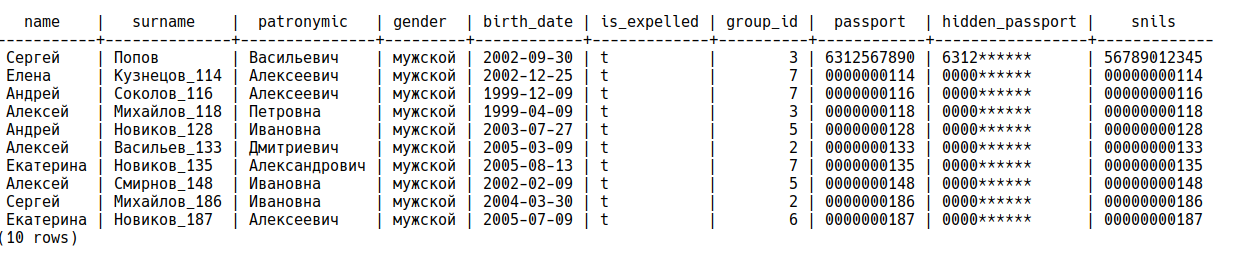
\includegraphics[scale=0.5]{q4p1.png}
\end{figure}

\item Получение кода представления:
\begin{minted}{sql}
SELECT pg_get_viewdef('view_students', true);
\end{minted}

\begin{figure}
\centering
 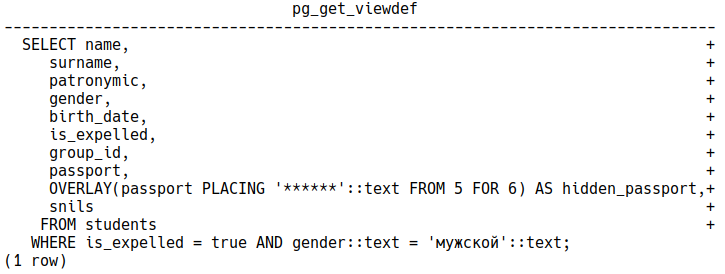
\includegraphics[scale=0.9]{q4p2.png}
\end{figure}

\item Запросы вставки и их результаты:

\begin{itemize}
\item Запрос 1:
\begin{minted}{sql}
INSERT INTO view_students (name, surname, patronymic, gender, birth_date, passport, snils, group_id, is_expelled)
VALUES ('Иванов', 'Алексей', 'Петрович', 'мужской', '2007-02-09', '6321254547', '6756891354', 1, FALSE);
\end{minted}

Студент не соответствует критериям представления (не отчислен). Это не позволяет выполнить вставку.

\begin{figure}
\centering
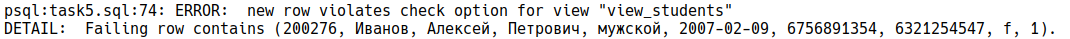
\includegraphics[scale=0.6]{q5p1.png}
\end{figure}

\item Запрос 2:
\begin{minted}{sql}
INSERT INTO view_students (name, surname, patronymic, gender, birth_date, passport, snils, group_id, is_expelled)
VALUES ('Петрова', 'Кристина', 'Олеговна', 'женский', '2005-04-24', '6320209823', '1234018745', 2, TRUE);
\end{minted}

Студент не соответствует критериям представления (не мужского пола). Это не позволяет выполнить вставку.

\begin{figure}
\centering
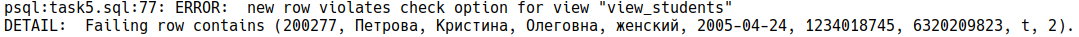
\includegraphics[scale=0.6]{q5p2.png}
\end{figure}

\item Запрос 3:
\begin{minted}{sql}
INSERT INTO view_students (name, surname, patronymic, gender, birth_date, passport, snils, group_id, is_expelled)
VALUES ('Ефимов', 'Станислав', 'Владимирович', 'мужской', '2006-05-12', '6320391768', '2395151234', 3, TRUE);
\end{minted}

Студент соответствует критериям представления. Это позволяет успешно выполнить вставку.

\begin{figure}
\centering
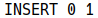
\includegraphics{q5p3.png}
\end{figure}
\end{itemize}
\end{enumerate}

\subsection{Базовое представление, использующееся в следующих представлениях}

\begin{minted}{sql}
CREATE OR REPLACE VIEW view_students AS
SELECT
  name, surname,
  patronymic,
  gender,
  birth_date,
  is_expelled,
  group_id,
  passport,
  OVERLAY (passport PLACING '******' FROM 5 FOR 6) AS hidden_passport,
  snils
FROM students
WHERE is_expelled = TRUE AND students.gender = 'мужской';
\end{minted}

\subsection{Представление с использованием LOCAL CHECK OPTION}

Опция LOCAL означает, что новые строки проверяются только по условиям, определённым непосредственно в самом представлении. Любые условия, определённые в нижележащих базовых представлениях, не проверяются (если только в них нет указания CHECK OPTION).

Код представления:

\begin{minted}{sql}
CREATE VIEW view_students_2007 AS
SELECT * FROM view_students
WHERE EXTRACT(YEAR FROM birth_date) = 2007
WITH LOCAL CHECK OPTION;
\end{minted}

Запросы вставки и их результаты:

\begin{itemize}
\item Запрос 1:
\begin{minted}{sql}
INSERT INTO view_students_2007 (name, surname, patronymic, gender, birth_date, passport, snils, group_id, is_expelled)
VALUES ('Иванов', 'Алексей', 'Петрович', 'мужской', '2007-02-09', '6321254507', '6756891394', 1, FALSE);
\end{minted}

Студент соответствует критериям представления (2007 года рождения), несмотря на то, что базовому представлению он не удовлетворяет (не отчислен). Это позволяет успешно выполнить вставку.

\begin{figure}
\centering
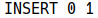
\includegraphics{q6p1.png}
\end{figure}

\item Запрос 2:
\begin{minted}{sql}
INSERT INTO view_students_2007 (name, surname, patronymic, gender, birth_date, passport, snils, group_id, is_expelled)
VALUES ('Петрова', 'Кристина', 'Олеговна', 'женский', '2005-04-24', '6320109813', '1254018735', 2, TRUE);
\end{minted}

 Студент не соответствует критериям текущего представления (не 2007 года рождения). Это не позволяет выполнить вставку.

\begin{figure}
\centering
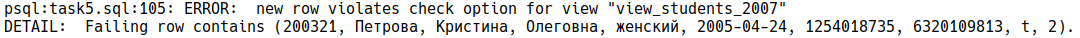
\includegraphics[scale=0.6]{q6p2.png}
\end{figure}
\end{itemize}

\subsection{Представление с использованием CASCADED CHECK OPTION}

Опция CASCADED  означает, что новые строки проверяются по условиям данного представления и всех нижележащих базовых.

Код представления:

\begin{minted}{sql}
CREATE VIEW view_students_2007_expelled AS
SELECT * FROM view_students1
WHERE EXTRACT(YEAR FROM birth_date) = 2007
WITH CASCADED CHECK OPTION;
\end{minted}

Запросы вставки и их результаты:

\begin{itemize}
\item Запрос 1:
\begin{minted}{sql}
INSERT INTO view_students_2007_expelled (surname, name, patronymic, gender, birth_date, passport, snils, group_id, is_expelled)
VALUES ('Иванов', 'Алексей', 'Петрович', 'мужской', '2007-02-09', '6321254567', '6756891254', 1, FALSE);
\end{minted}

Студент соответствует критериям текущего представления (2007 года рождения), однако не соответствует критериям базового представления (не отчислен). Это не позволяет выполнить вставку.

\begin{figure}
\centering
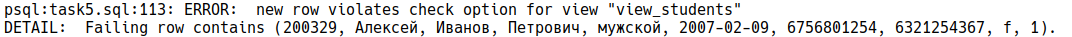
\includegraphics[scale=0.6]{q7p1.png}
\end{figure}

\item Запрос 2:
\begin{minted}{sql}
INSERT INTO view_students_2007_expelled (surname, name, patronymic, gender, birth_date, passport, snils, group_id, is_expelled)
VALUES ('Афоничев', 'Иван', 'Алексеевич', 'мужской', '2007-01-13', '632125172', '1332067854', 3, TRUE);
\end{minted}

Студент соответствует критериям текущего представления (2007 года рождения), а  также всем критериям базового представления (мужского пола, отчислен). Это позволяет успешно выполнить вставку.

\begin{figure}
\centering
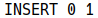
\includegraphics{q7p2.png}
\end{figure}
\end{itemize}

\section{Индексированные представления}

Работать с индексами в представлении можно только если оно материализированное. Это достигается с помощью добавления модификатора MATERIALIZED при создании представления.

Нужно создать индекс для представления, а далее сравнить производительность индексированного представления с производительностью запроса SELECT, на котором оно основано.

\begin{enumerate}
\item Код представления:
\begin{minted}{sql}
CREATE MATERIALIZED VIEW view_student_orders AS
SELECT
  students.id,
  students.surname,
  students.name,
  COUNT(student_orders.id) AS order_count,
  MAX(student_orders.order_date) AS last_order
FROM students
LEFT JOIN student_orders ON students.id = student_orders.student_id
GROUP BY students.id, students.surname, students.name;
\end{minted}

\item Запрос SELECT, на котором основано представление:
\begin{minted}{sql}
EXPLAIN ANALYZE
SELECT
  students.id,
  students.surname,
  students.name,
  COUNT(student_orders.id) AS order_count,
  MAX(student_orders.order_date) AS last_order
FROM students
LEFT JOIN student_orders ON students.id = student_orders.student_id
WHERE students.surname LIKE 'Иванов%'
GROUP BY students.id, students.surname, students.name;
\end{minted}

\item Скриншот плана выполнения запроса:
\begin{figure}
\centering
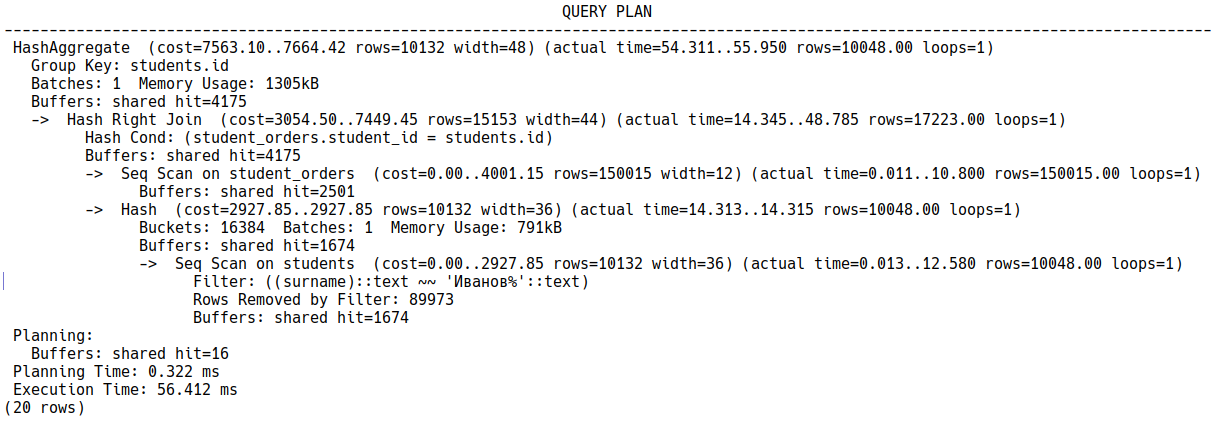
\includegraphics[scale=0.6]{q8p1.png}
\end{figure}

\item Индекс, разработанный для представления:
\begin{minted}{sql}
CREATE INDEX idx_order_surname ON view_student_orders(surname varchar_pattern_ops);
\end{minted}

\item Аналогичный запрос SELECT, но уже к представлению:
\begin{minted}{sql}
CREATE INDEX idx_order_surname ON view_student_orders(surname varchar_pattEXPLAIN ANALYZE
SELECT * FROM view_student_orders
WHERE surname LIKE 'Иванов%';
\end{minted}

\item Скриншот плана выполнения запроса с индексом:
\begin{figure}
\centering
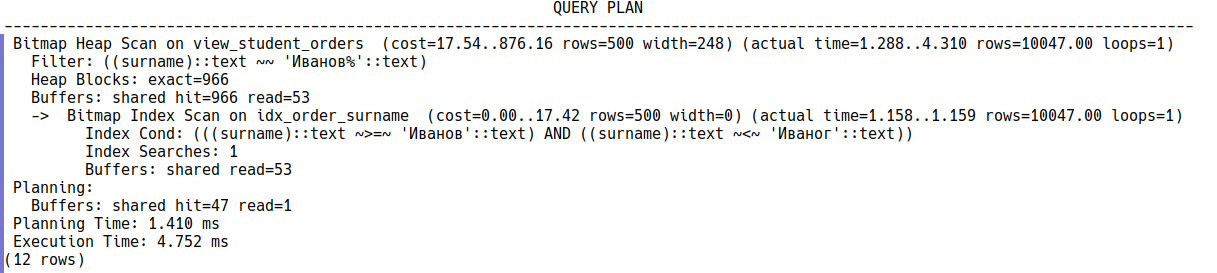
\includegraphics[scale=0.6]{q8p2.png}
\end{figure}

Можно увидеть, что сочетание представления и индекса в значительной степени ускорило данный запрос.
\end{enumerate}
%После введения — серии \section, \subsection и т.д.

% \conclusion

% Отобразить все источники. Даже те, на которые нет ссылок.
% \nocite{*}

\bibliographystyle{ugost2008}
\bibliography{thesis}

% Окончание основного документа и начало приложений Каждая последующая секция
% документа будет являться приложением
\appendix

\end{document}
